\documentclass[letterpaper]{article} % DO NOT CHANGE THIS
\usepackage[submission]{aaai2027}  % DO NOT CHANGE THIS
\usepackage[hyphens]{url}  % DO NOT CHANGE THIS
\urlstyle{rm} % DO NOT CHANGE THIS
\def\UrlFont{\rm}  % DO NOT CHANGE THIS
\usepackage{natbib}  % DO NOT CHANGE THIS AND DO NOT ADD ANY OPTIONS TO IT
\usepackage{caption} % DO NOT CHANGE THIS AND DO NOT ADD ANY OPTIONS TO IT
\frenchspacing  % DO NOT CHANGE THIS
\pdfinfo{/TemplateVersion (2027.1)}
\setcounter{secnumdepth}{0}

\usepackage[utf8]{inputenc}
\usepackage[T1]{fontenc}
\usepackage{booktabs}
\usepackage{amsfonts}
\usepackage{amsmath}
\usepackage{amssymb}
\usepackage{bbm}
\usepackage{nicefrac}
\usepackage{microtype}
\usepackage{graphicx}
\usepackage{xcolor}
\usepackage{multirow}
\usepackage{array}
\usepackage{subcaption}

\graphicspath{{figures/}}

\renewcommand{\topfraction}{0.9}
\renewcommand{\bottomfraction}{0.8}
\renewcommand{\textfraction}{0.07}
\renewcommand{\floatpagefraction}{0.7}
\setcounter{topnumber}{3}
\setcounter{bottomnumber}{2}
\setcounter{totalnumber}{4}

\title{ReGainX: Adaptive Reinforcement Learning Exoskeletons\\
for Real-Time Mitigation of Parkinson's Motor Impairments}

% Anonymous submission — author block omitted per AAAI blind-review policy.
% For camera-ready, replace with:
%   \author{Rohan Bankapur}
%   \affiliations{Independent Researcher\\Frisco, TX, USA\\rohannb02@gmail.com}
\author{Anonymous}
\affiliations{Anonymous Institution}

\begin{document}
\maketitle

% ─────────────────────────────────────────────────────────────────────────────
\begin{abstract}
Parkinson's disease (PD), consisting of muscular degeneration and bradykinesia,
weakens daily elbow movement for millions and still remains largely unaddressed.
State-of-the-art exoskeletons fail to generalize to the erratic Parkinson's
symptoms due to a lack of datasets and calibration difficulty.
ReGainX introduces a hierarchical reinforcement learning (Hierarchical RL) pipeline to
train diverse, synthetic PD digital twins and an elbow exoskeleton controller, both via
Proximal Policy Optimization (PPO).
Via an LSTM feature extractor, every 5\,ms, the controller uses the patient's simulated
muscle-activation and joint-state observations to estimate movement intent and impairment
state, and provides assistive torque.
Our policy achieved, on average, a correlation of 0.494 with the healthy elbow
movement and a task completion rate of 88.8\%, without recalibration.
An ablation study revealed a 35.7\% higher trajectory match over a policy trained on
muscular degeneration alone---mirroring the dominant approach in current exoskeletons,
which do not account for bradykinesia---confirming this is insufficient for patients
experiencing both PD impairments simultaneously.
Through deploying state-of-the-art control policies and constructing a
high-fidelity environment modelling Parkinson's Disease motor impairments, our
work paves a scalable pathway for transferring simulation-trained deep
reinforcement learning policies to real-world, generalisable assistive devices.
\end{abstract}

\keywords{Parkinson's disease, exoskeleton, reinforcement learning,
musculoskeletal simulation, bradykinesia, hierarchical reinforcement learning}

% =============================================================================
\section{Introduction}
\label{sec:intro}

Parkinson's disease (PD) affects over 10 million people, costing the
U.S.\ \$82.2 billion annually~\citep{chaudhuri2025, parkinson2026}.
PD can restrict the elbow through two impairments: \emph{muscular degeneration},
the progressive weakening of muscles, and \emph{bradykinesia}, the slowness and
delay of voluntary movement.
This restriction can vary from patient to patient, often cycling between states
in a single day as variables such as medication and physical activity
fluctuate~\citep{ramesh2022}.
However, even mildly affected PD patients have shown a reduced force at the
elbow by 22\%~\citep{ingram2021}.

\begin{figure}[tbp]
  \centering
  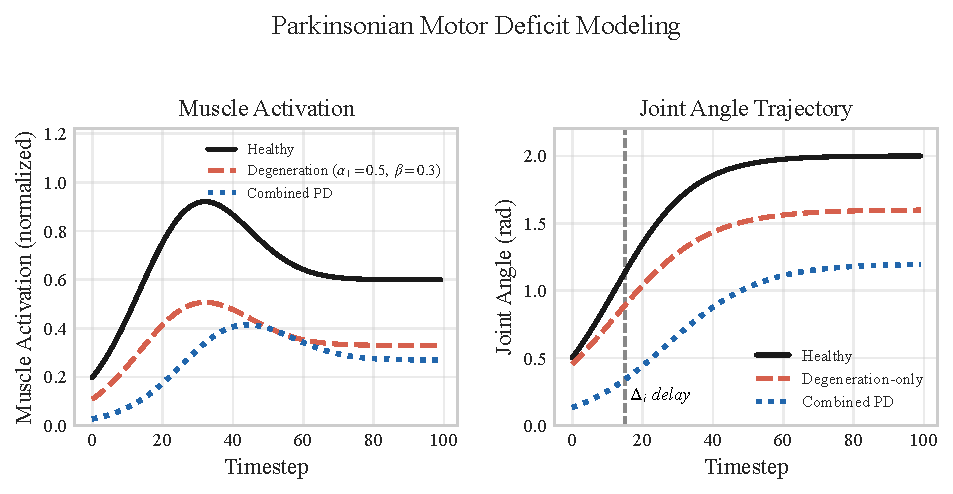
\includegraphics[width=\linewidth]{fig2_pd_modeling.pdf}
  \caption{Healthy vs.\ Parkinsonian elbow movement.
    \textbf{Left:} Muscle activation is reduced by degeneration and further
    delayed under combined PD impairment.
    \textbf{Right:} Joint-angle trajectories show reduced reach and delayed
    onset; the vertical dashed line marks the akinetic delay $\Delta i$.}
  \label{fig:elbow}
\end{figure}

Current PD-assistive wearables often fail to meet patients' needs on three
fronts: the reliance on heavy, frequent, and manual calibration; sensor noise;
and limited transferability between different patients due to the lack of
PD-specific datasets~\citep{researchgate2023, caggiano2022}.
This is reflected by the 82\% deficit of PD patients actually adopting these
wearables, from the 90\% interest in this technology~\citep{hirczy2024}.

Elbow exoskeletons have been constantly evolving, with the first elbow
exoskeletons using rigid trajectory control.
Although this did offer assistance, the inflexible controller interrupted natural
movement, forcing the joint across a fixed path regardless of user effort,
impairment, and position~\citep{gasperina2021, myoelectric2022}.
\citet{supriyono2025} confirm this, finding that the elbow joint is a crucial
joint for upper-limb movement, but control models often require patient- and
session-specific parameters and tuning.
However, this tuning introduces a barrier to adoption for PD patients who face
short-term and long-term fluctuations.
Therefore, because tuning is a hurdle for many users, not only those facing PD,
research has shifted towards an ``intent-detection'' based approach using
myoelectric signals.
Predominantly through machine learning, data analysis of EMG
(Electromyography) on targeted muscles allows devices to capture movement
intention and muscle activation state.
However, surface EMG remains noisy, exacerbating PD's basal ganglia dysfunction,
introducing a tradeoff through invasive sensors and
effectiveness~\citep{supriyono2025, mdpi2025}.

Deep Reinforcement Learning (DRL) control policies reduce the need for
calibration of exoskeletons.
State-of-the-art RL control policies for exoskeletons are trained through
interacting with a distribution of simulated patients, rather than just tuning
to one real patient.
In fact, \citet{luo2024} deployed, with sim-to-real transfer, a general DRL hip
exoskeleton which resulted in a 24.3\% metabolic walking effort reduction.
Despite the effectiveness, there still remains a gap in applying exoskeletons
for PD, attributed to the absence of IMU and EMG data for PD assistive devices.
However, DRL has been applied specifically to PD, demonstrating tremor
suppression and adaptation across severities and
movements~\citep{endrei2025}.
No prior work has established an autonomous elbow exoskeleton controller for
PD motor symptoms.
Additionally, the lack of datasets makes simulation necessary, inherently
guiding PD-based exoskeleton controllers towards Online DRL, but no existing
PD environments have been constructed for exoskeletons.

ReGainX addresses this gap with a multi-agent DRL framework.
Through MyoSuite's high-fidelity musculoskeletal simulator, we train a healthy
digital twin of the human elbow via DRL, then apply randomised severities of PD
symptoms to generate a distribution of PD digital twins, and then we train a DRL
exoskeleton agent against the $\approx$20,000 distinct PD digital twins.
In this paper, we question whether deep reinforcement learning can produce an
autonomous elbow exoskeleton environment and controller that provides real-time
adaptive mitigation of PD motor impairments at the elbow.

% =============================================================================
\section{Related Work}
\label{sec:related}

\subsection{Control Models for Elbow Exoskeletons}

The first elbow exoskeletons assisted with forces independent of human movement,
often disrupting movements and proving inadequate for patients with fluctuating
impairment severities~\citep{gasperina2021}.
Then, elbow exoskeleton control mechanisms evolved to detect human intention
through surface EMG (sEMG) and IMU sensing, as deep learning evolved.
Now, they serve as a state-of-the-art mechanism for exoskeletons because of
their low cost and high information density~\citep{supriyono2025}.
Despite their effectiveness, sensor noise and patient-specific models are the
primary barriers to preventing cross-patient
generalisation~\citep{supriyono2025}.

\subsection{Exoskeletons for Parkinson's Disease}

Despite PD being a common motor disorder, established exoskeleton work targeting
PD patients is sparse.
A systematic review of exoskeletons for PD found only five studies, involving
46 patients total, all on stable medication and at Hoehn \& Yahr stages below
3~\citep{fortunati2024}.
However, none of these exoskeletons adopted adaptive control or covered the
upper limb; the elbow, a major site of PD motor decline, has not been targeted
in existing works.

\subsection{Deep Reinforcement Learning for Exoskeleton Control}

Due to the limitation of static, patient-calibrated controllers for exoskeletons,
work has shifted towards deploying DRL as the primary control policy.
\citet{luo2023} presented one of the first DRL-based controllers for lower-limb
exoskeletons.
Additionally, they trained their exoskeleton via musculoskeletal simulators,
adopting domain randomisation for muscle strength across quadriplegic,
muscle-weakness, and hemiplegic conditions and then deployed it,
experiment-free.
Additionally, \citet{endrei2025} utilised DRL for PD tremor suppression,
showing DRL's capability in accounting for the severity fluctuations
characterising PD.
However, none of these works simulate muscular degeneration and bradykinesia,
two defining factors of PD at the elbow.

\subsection{Musculoskeletal Simulators as an Environment}

The absence of assistance-related PD datasets at the elbow makes high-fidelity
simulation the most feasible approach.
\citet{caggiano2022} introduced MyoSuite, a rich musculoskeletal simulator built
upon MuJoCo by modelling physiological impairments, including fatigue and
sarcopenia, and setting up environments and meshes for task training.
\citet{wang2022} extended this with MyoSim, streamlining the process, making
large episode counts more computationally feasible and faster.
However, there is a large absence in work that has been able to apply these
capabilities to simulate PD and train an elbow exoskeleton controller.

% =============================================================================
\section{Parkinson's Disease Simulation}
\label{sec:pdsim}

\subsection{Musculoskeletal Model}

We construct our digital twins in MyoSuite's \texttt{myoElbow} environment, a
6-muscle elbow model (three primary flexors and extensors) deployed on
MuJoCo~\citep{caggiano2022}.
Muscle force follows Hill-type muscle-tendon dynamics, which depends on current
muscle activation, fibre operating length, and
contraction~\citep{zajac1989}.
Joint torque can be represented through the following equation:
\begin{equation}
  \boldsymbol{\tau} = M(\mathbf{q})\ddot{\mathbf{q}}
    + C(\mathbf{q}, \dot{\mathbf{q}})\dot{\mathbf{q}}
    + G(\mathbf{q}),
  \label{eq:torque}
\end{equation}
where $M(\mathbf{q})$ serves as the inertia matrix,
$C(\mathbf{q}, \dot{\mathbf{q}})$ accounts for Coriolis and centrifugal forces,
and $G(\mathbf{q})$ is the gravity vector.
The elbow joint's range of motion is limited to $2.4\,\mathrm{rad}$
($\approx$138$^\circ$), consistent with the established elbow movement
ranges~\citep{cools2017, morrey1981}.
The exoskeleton provides a normalised torque
$\tau_\text{exo}\in[0,1]$, proportional to the biological joint torque
capacity~\citep{durandau2019}.

The elbow extensors show the biggest gap in force production (22\%), even in
mild PD severities~\citep{ingram2021}, and the movement is essential for daily
tasks such as eating or drinking.
Limitations in the elbow significantly restrict elbow flexion velocity and range
of motion~\citep{caligiuri2018}.

\subsection{Muscular Degeneration Model}

Muscular degeneration is prevalent in PD through sarcopenia (with 10.9--31.4\%
of patients facing it) and chronic muscular fatigue
($\approx$50\%)~\citep{hart2023, ponsoni2023, siciliano2024}.
We use MyoSuite's existing degeneration equations and
framework~\citep{caggiano2022}:
\begin{equation}
  F_\text{deg} = \alpha_1 \cdot F_\text{max}
    \cdot e^{-(\alpha_2 + \beta t)}
    = m_\text{loss} \cdot m_\text{fati},
  \label{eq:degeneration}
\end{equation}
where $\alpha_1\in[0,1]$ is the sarcopenia mass-loss parameter,
$\alpha_2\in[0,1]$ is the fatigue rate parameter, and $\beta$ is MyoSuite's
default value from \citeauthor{caggiano2022}'s (2020) three-compartment fatigue
model.
All parameters are independently randomised per episode, forcing our policy to
adapt to different configurations of muscular degeneration and fatigue severity.

\subsection{Bradykinesia Model}

Bradykinesia is characterised by two symptoms: a delay in movement initiation
and a reduction in movement speed and magnitude.
PD patients off medication move 41\% slower and have 29\% shorter
displacement~\citep{agostino2015}.
We model bradykinesia as:
\begin{equation}
  N_\text{brady} = x(i - \Delta i) \cdot \alpha,
  \label{eq:bradykinesia}
\end{equation}
where $\Delta i\in[1.1,\,1.4]$ is a temporal scaling factor (an action
taking 1.0\,s healthy takes 1.1--1.4\,s in a PD patient) and
$\alpha\in[0.3,\,1.0]$ scales the movement amplitude, representing the
29--41\% reduction documented clinically from medicated vs.\ non-medicated
patients~\citep{agostino2015, raethjen2018}.
$\alpha$ extends beyond the documented clinical deficit because
\citeauthor{agostino2015}'s measurements were taken relative to medicated
patients, who may already carry residual deficits compared to healthy controls.

\subsection{Combined PD Severity and Episode Diversity}

Muscular degeneration and bradykinesia modelling is applied across all training
episodes.
Our framework randomises symptom-specific parameters---impairment levels,
noise, start angle, and target goal angle (both over $0$--$2.4\,\mathrm{rad}$).
Therefore, the policy encounters no two identical patient profiles during
training, requiring our model to generalise to a wide range of PD severities.

% =============================================================================
\section{Methodology}
\label{sec:method}

\subsection{Safety Design}
\label{sec:safety}

MyoSuite's exoskeleton model incorporates an upper-arm attachment
($0.101\,\mathrm{kg}$) and a forearm attachment ($0.111\,\mathrm{kg}$), falling
in the range of $0.2$--$0.5\,\mathrm{kg}$ for attachments that are comfortable
for patients with reduced arm strength~\citep{pmc11852623, pmc12451468}.
To verify that the upper-limb attachments cannot harm movement when not providing
assistance, an experiment was conducted in which the healthy elbow was evaluated
with and without the weight of the exoskeleton.
We found a strong trajectory match, confirming that the weight does not interfere
with voluntary movement.

ReGainX enforces two safety constraints.
First, the joint angle of the exoskeleton is capped at $2.4\,\mathrm{rad}$, the
established upper limit for elbow flexion~\citep{cools2017}.
Exoskeleton torque is also normalised to $[0,1]$ as a fraction of biological
joint torque.
The exoskeleton cannot deliver more torque than the joint's own biological
capacity.

\subsection{Hierarchical RL Training Framework}
\label{sec:marl}

ReGainX implements a three-phase hierarchical RL pipeline
(Figure~\ref{fig:pipeline}) to develop a healthy musculoskeletal elbow
controller, a simulated PD patient, and an exoskeleton controller.
The hierarchy is enforced by freezing the patient controller before exoskeleton
training begins; concurrent training would allow the patient model to drift
toward unnatural movement patterns that inflate the shared reward.
ReGainX is structured so the exoskeleton must adapt to the patient, not vice versa,
and the patient controller's learned behaviour is held fixed as a stationary
environment for the exoskeleton policy.

\begin{figure}[tbp]
  \centering
  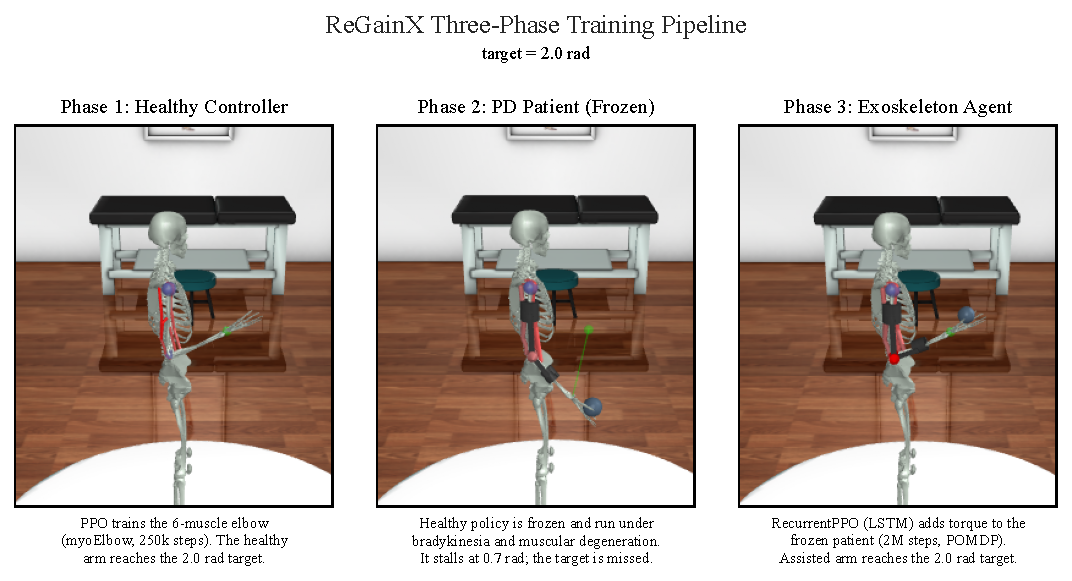
\includegraphics[width=\linewidth]{fig1_pipeline.pdf}
  \caption{Three-phase ReGainX training pipeline.
    \textbf{Phase 1:} A PPO healthy controller drives the six elbow muscles and
    reaches the target.
    \textbf{Phase 2:} The same controller is frozen and run under combined
    bradykinesia and muscular degeneration, stalling short of the target.
    \textbf{Phase 3:} A RecurrentPPO exoskeleton agent supplies assistive torque
    to the frozen patient, restoring movement to the target.}
  \label{fig:pipeline}
\end{figure}

\paragraph{Phase 1 --- Healthy Controller Training.}
A musculoskeletal elbow controller is trained on MyoSuite's 6-muscle elbow pose
environment via PPO~\citep{sb3} for 250\,000 timesteps.
The action space is the 6-dimensional neural drive signal.
The per-timestep reward measures how much closer the current joint angle $q_t$
has moved towards the target angle $q^*$.
The elbow must learn to move between starting and target angles drawn randomly
from $[0,\,2.4]\,\mathrm{rad}$ each episode.
The pose-error reward used throughout training and evaluation is MyoSuite's
built-in \texttt{get\_reward\_dict} for the pose environment~\citep{caggiano2022}:
\begin{equation}
  r_t = -\lVert \mathbf{e}_t \rVert_2
      + 4\Bigl[\mathbbm{1}(\lVert \mathbf{e}_t \rVert_2 < \theta)
             + \mathbbm{1}(\lVert \mathbf{e}_t \rVert_2 < 1.5\theta)\Bigr]
      - \frac{\lVert \mathbf{a}_t \rVert_2}{n_a}
      - 50\cdot\mathbbm{1}(\lVert \mathbf{e}_t \rVert_2 > 2\pi),
  \label{eq:reward_phase1}
\end{equation}
where $\mathbf{e}_t = q^* - q_t$ is the joint angle error,
$\theta = 0.175\,\mathrm{rad}$ is MyoSuite's default pose tolerance,
$\mathbf{a}_t$ is the muscle activation vector,
$n_a$ is the number of actuators, and
$\mathbbm{1}(\cdot)$ is the indicator function.
The two bonus thresholds ($\theta$ and $1.5\theta$) are hardcoded in MyoSuite's
reward function and were not modified.

\paragraph{Phase 2 --- Parkinson's Patient Controller Setup.}
The healthy elbow controller is transferred to a new environment.
Implementing the modelling equations discussed in
Section~\ref{sec:pdsim}, joint position errors increase as a realistic impaired
profile is created.
As an alternative to real PD datasets, which are scarce, we randomise impairment
parameters to create $\approx$20\,000 distinct patient profiles in simulation.

\paragraph{Phase 3 --- Exoskeleton Agent Training.}
With the PD controller frozen in the environment, the exoskeleton controller is
initialised and trained for 2\,000\,000 timesteps using RecurrentPPO.
Both the elbow and the exoskeleton act each timestep.
The exoskeleton agent receives an 8-dimensional observation---the patient's
6 simulated muscle activations and 2 joint-state values ($q_t$, $\dot{q}_t$,
described fully in \S\ref{sec:policy})---and outputs a single normalised
torque value $\tau_\text{exo}\in[0,1]$.
Its objective is to maximise the exoskeleton pose-error reward:
\begin{equation}
  r_t^{\text{exo}} = -\lVert \mathbf{e}_t \rVert_2
      + 4\Bigl[\mathbbm{1}(\lVert \mathbf{e}_t \rVert_2 < 0.175)
             + \mathbbm{1}(\lVert \mathbf{e}_t \rVert_2 < 0.2625)\Bigr]
      - 5\cdot\frac{\lVert \mathbf{a}_t \rVert_2}{n_a}
      - 50\cdot\mathbbm{1}(\lVert \mathbf{e}_t \rVert_2 > 2\pi),
  \label{eq:reward_exo}
\end{equation}
which is identical to Equation~\ref{eq:reward_phase1} except the activation
regularisation weight is increased from $1.0$ to $5.0$, penalising the
exoskeleton more heavily for unnecessary torque output (the exoskeleton should
assist, not override, the patient's residual muscle activity).

To satisfy the Markov property, the observation space consists of the 6 muscle
activations produced by the frozen patient controller (the simulation's analogue
to surface EMG signals), the current joint angle $q_t$, and the current joint
velocity $\dot{q}_t$ (the simulation's analogue to IMU-derived kinematics).
Velocity encodes the change of the joint state without requiring access to prior
states.
The target angle is deliberately excluded: it is not feasible to require a patient
to specify a precise target angle before every movement, so the LSTM must infer
intended direction from the unfolding activation pattern.

\subsection{Policy Architecture}
\label{sec:policy}

ReGainX's primary exoskeleton policy is a RecurrentPPO~\citep{sb3contrib}, which
adds an LSTM layer before the PPO actor-critic framework to extract temporal
context from the observation input.
Each timestep, the LSTM uses a cell state and hidden state carried forward within
an episode.
Each episode, the policy re-initialises its temporal context per patient profile.
Our training framework trades off long-term temporal context, which would require
longer episodes, for cheaper training.

The control problem can be framed as a Partially Observable Markov Decision
Process (POMDP).
Our observation space excludes the target angle because it is not feasible for
the user to input this angle for every task.
Therefore, the LSTM layers must extract information across the patient's
activation pattern and joint movement to infer intended movement direction and
the degree to which impairment will prevent its completion.
Through introducing temporal context, our policy is able to distinguish
impairment and movement progression.

The shorter rollout of 256 steps was used to produce frequent LSTM state resets
during training, to avoid vanishing gradients and amplify the episode boundary
signal.
The training reward curves for all policies are shown in
Figure~\ref{fig:training}.

\begin{figure}[tbp]
  \centering
  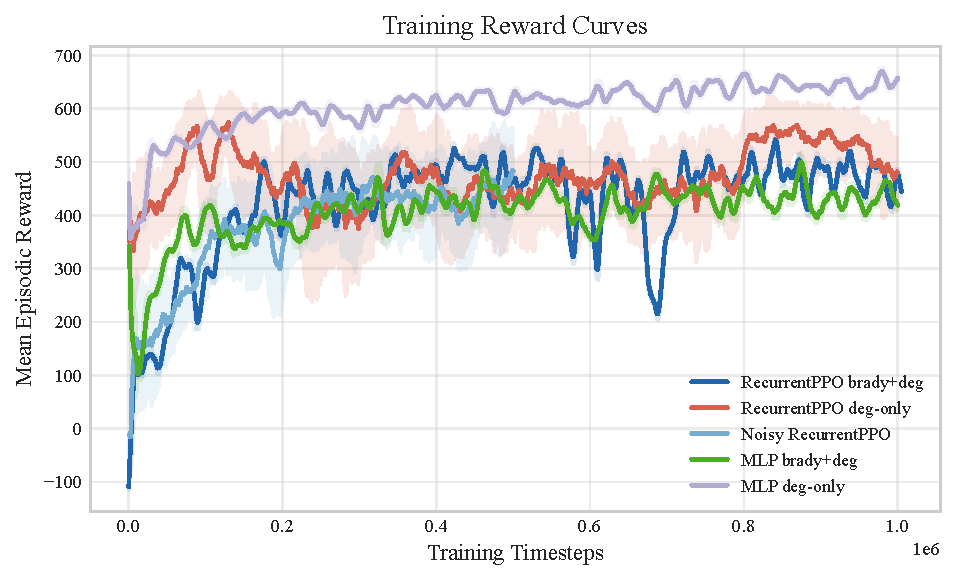
\includegraphics[width=\linewidth]{fig3_training_curves.pdf}
  \caption{Training reward curves (rolling mean, window~$=20$, with
    $\pm1\sigma$ band).
    The RecurrentPPO brady+deg policy converges substantially more slowly than
    MLP policies, consistent with the higher sample complexity of learning a
    useful LSTM hidden state.}
  \label{fig:training}
\end{figure}

\subsection{Hyperparameter Optimisation}
\label{sec:hparam}

Hyperparameters were tuned via Bayesian Optimisation~\citep{akiba2019} with a
Tree-structured Parzen Estimator (TPE) sampler and a MedianPruner (5 startup
trials and 2 warmup steps).
We ran two hyperparameter tuning sessions, one for the MLP baseline and one for
the RecurrentPPO.
We ran each for 1\,500\,000 timesteps with a 10-episode evaluation per trial.
The best configurations and study statistics are listed in Table~\ref{tab:bayes}.

\begin{table}[tbp]
  \centering
  \caption{Bayesian optimisation results.}
  \label{tab:bayes}
  \begin{tabular}{lcc}
    \toprule
    \textbf{Metric} & \textbf{MLP} & \textbf{RecurrentPPO} \\
    \midrule
    Completed / pruned trials & 13 / 7 & 11 / 9 \\
    Reward range & $-62.88$--$546.37$ & $27.67$--$377.07$ \\
    Mean reward  & $367.14 \pm 190.40$ & $143.91 \pm 89.87$ \\
    Best learning rate & $9.31\times10^{-4}$ & $7.90\times10^{-5}$ \\
    Best $n_\text{steps}$ & 512 & 4096 \\
    Best batch size & 256 & 64 \\
    Best entropy coef & $0.01641$ & $1.96\times10^{-4}$ \\
    Best $\gamma$ & $0.9986$ & $0.9835$ \\
    Best clip range & $0.2320$ & $0.2320$ \\
    \bottomrule
  \end{tabular}
\end{table}

\subsection{Inference Latency}
\label{sec:latency}

Inference latency for the policies was measured over 1\,000 timed forward
passes.
Results are shown in Figure~\ref{fig:latency} and Table~\ref{tab:latency}.
Although the RecurrentPPO had an additional LSTM layer, it produced a mean
inference latency of $1.930\,\mathrm{ms}$---well below the 10--20\,ms control
period of typical upper-limb exoskeletons~\citep{supriyono2025}.

\begin{figure}[tbp]
  \centering
  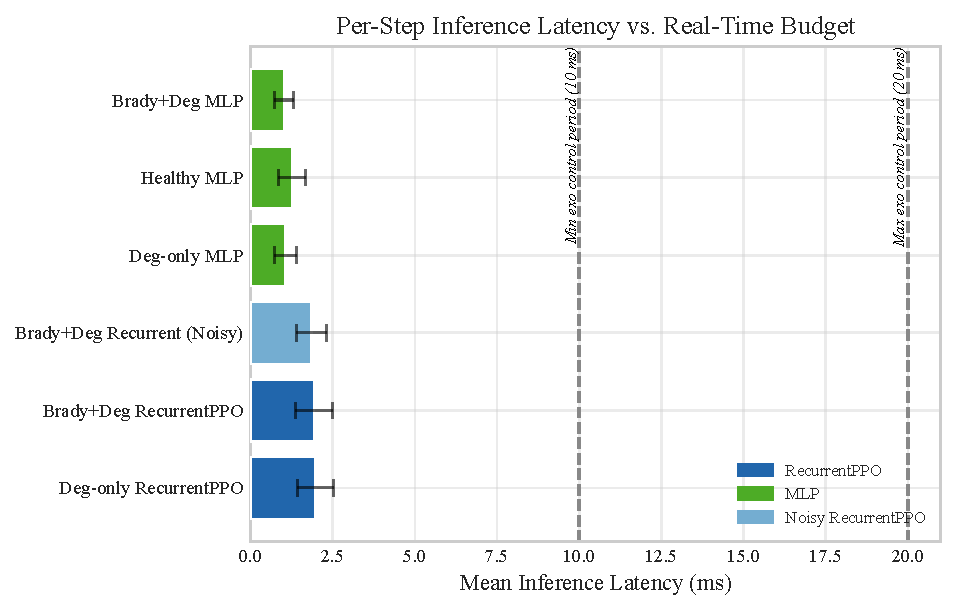
\includegraphics[width=\linewidth]{fig8_latency.pdf}
  \caption{Per-step inference latency (mean~$\pm$ std) for each policy.
    Vertical lines mark the 10--20\,ms exoskeleton real-time control budget;
    all policies run well within budget.}
  \label{fig:latency}
\end{figure}

\begin{table}[tbp]
  \centering
  \caption{Inference latency across architectures (ms).}
  \label{tab:latency}
  \small
  \begin{tabular}{lrrrrrrr}
    \toprule
    \textbf{Model} & \textbf{Mean} & \textbf{Std} & \textbf{Min}
      & \textbf{p5} & \textbf{p50} & \textbf{p99} & \textbf{Max} \\
    \midrule
    Healthy MLP               & 1.267 & 0.405 & 0.840 & 0.896 & 1.090 & 2.414 & 2.799 \\
    Brady+Deg MLP             & 1.017 & 0.302 & 0.807 & 0.827 & 0.902 & 2.412 & 2.704 \\
    Deg-only MLP              & 1.056 & 0.335 & 0.808 & 0.832 & 0.913 & 2.252 & 3.275 \\
    \textbf{Brady+Deg RecPPO} & \textbf{1.930} & \textbf{0.560}
      & \textbf{1.448} & \textbf{1.488} & \textbf{1.686}
      & \textbf{3.714} & \textbf{5.310} \\
    Noisy RecPPO              & 1.851 & 0.458 & 1.447 & 1.479 & 1.666 & 3.387 & 4.110 \\
    Deg-only RecPPO           & 1.974 & 0.555 & 1.454 & 1.495 & 1.752 & 3.960 & 4.887 \\
    \bottomrule
  \end{tabular}
\end{table}

% =============================================================================
\section{Experiments and Results}
\label{sec:results}

\subsection{Evaluation Methodology}

Our policies were evaluated across the same 4\,000 patient profiles.
Episodes were stratified across impairment severities (Q1--Q4) and ranges of
radians travelled by the elbow.
For every episode, three policies were run: a healthy elbow baseline, an impaired
patient with no exoskeleton, and the impaired patient with exoskeleton
assistance.

The primary metric used was the Pearson correlation coefficient $r$ of the
exoskeleton-assisted trajectory vs.\ the healthy baseline trajectory.
The healthy trajectory represents what the PD patient intended to do, but
impairment degrades execution.

As a secondary metric, we measured the goal achievement rate: the fraction of
episodes in which the target angle was reached.
Mean episodic reward is reported for policy comparisons.
All policies were trained to maximise the pose-error reward defined in
Equation~\ref{eq:reward_phase1}.

\subsection{Movement Restoration Performance}

Our primary policy---RecurrentPPO trained on combined PD impairments---achieved
$r{=}0.494$ (std~$=0.317$) and a goal rate of 88\%.
Relative to the no-exoskeleton baseline ($r{=}0.223$, goal rate~$=65.1\%$),
this improved the trajectory match by 0.271 and the goal rate by 23.7\%.
The mean reward improved from 97.37 to 499.73.

Across severity quartiles, trajectory match and goal rate degraded as the
exoskeleton's normalised torque ceiling became insufficient at more severe
impairments.

Across radians travelled, trajectory match increased as movements became longer.
This can be attributed to the LSTM layer's ability to accumulate temporal context
from more timesteps, improving intent and impairment assessment.
Figure~\ref{fig:heatmap} shows the full $4\times4$ performance heatmap.

\begin{figure}[tbp]
  \centering
  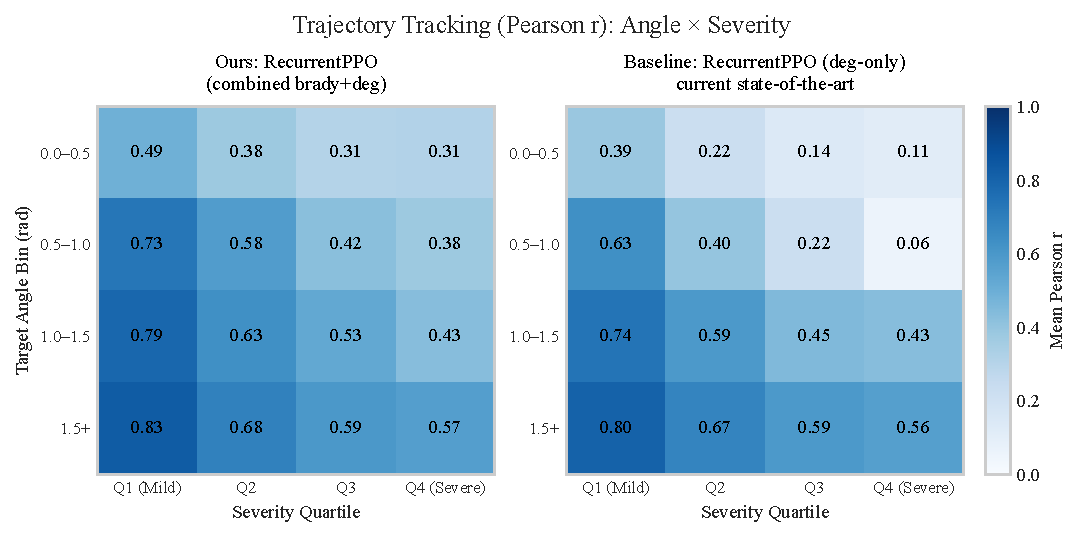
\includegraphics[width=\linewidth]{fig5_heatmap.pdf}
  \caption{Mean Pearson $r$ across target-angle bins (rows) and severity
    quartiles (columns) for the combined-trained RecurrentPPO (\textbf{left})
    versus the degeneration-only policy (\textbf{right}).}
  \label{fig:heatmap}
\end{figure}

\subsection{Ablation 1: RecurrentPPO vs.\ MLP}

Our primary policy, RecurrentPPO, achieved $r{=}0.494$ compared to the MLP's
$r{=}0.439$ across the 4\,000 patient profiles.
Goal rates were close (88.8\% vs.\ 89.0\%), but RecurrentPPO had a higher mean
reward (499.72 vs.\ 460.29), suggesting the policy had a smoother, more
proportionate trajectory toward the goal pose.
The MLP stabilised early at 512 timesteps, while the RecurrentPPO varied through
the full run, confirming the higher sample complexity of learning a useful hidden
state.
Figure~\ref{fig:ablation1} compares the two approaches across severity quartiles.

\begin{figure}[tbp]
  \centering
  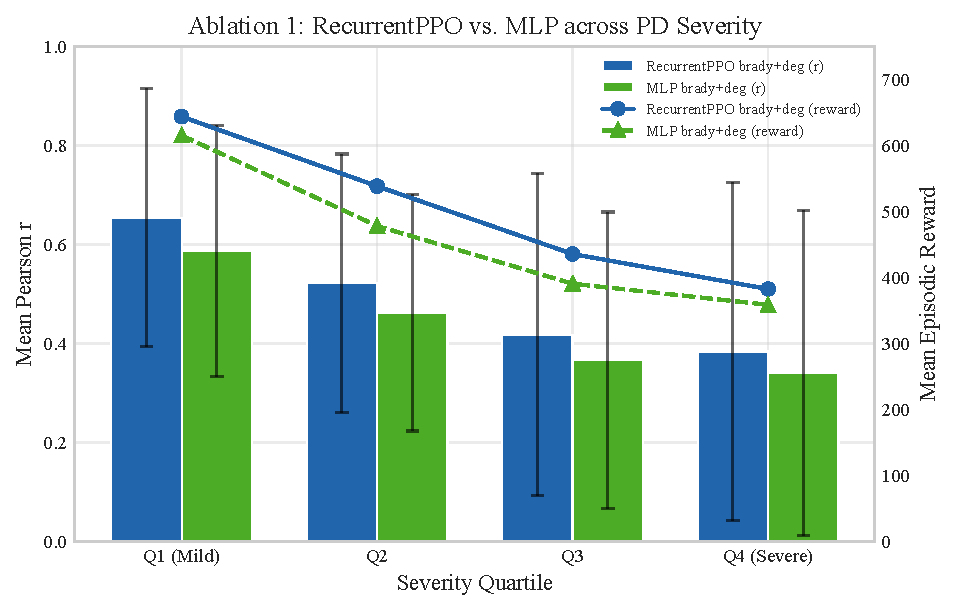
\includegraphics[width=\linewidth]{fig9_ablation1.pdf}
  \caption{Ablation 1: per-severity Pearson $r$ (bars) and mean episodic reward
    (lines) for RecurrentPPO brady+deg vs.\ MLP brady+deg.
    RecurrentPPO retains higher trajectory match and reward across all severity
    quartiles.}
  \label{fig:ablation1}
\end{figure}

\subsection{Ablation 2: Combined Impairment vs.\ Degeneration-Only Training}

Existing upper-limb exoskeleton control policies are predominantly tuned to
compensate for muscular weakness or degeneration alone; bradykinesia is not
modelled~\citep{gasperina2021, supriyono2025}.
The degeneration-only policy in this ablation therefore represents the closest
simulation of current practice.
Training on muscular degeneration alone will produce a policy that fails under
the full complexity of PD, as our experiments in Table~\ref{tab:ablation2} and
Figure~\ref{fig:ablation2} demonstrate.

\begin{table}[tbp]
  \centering
  \caption{Ablation 2: RecurrentPPO brady+deg vs.\ deg-only, evaluated on the
    full brady+deg environment.}
  \label{tab:ablation2}
  \begin{tabular}{lcccc}
    \toprule
    \textbf{Quartile} & \multicolumn{2}{c}{\textbf{Pearson $r$}}
      & \multicolumn{2}{c}{\textbf{Mean Reward}} \\
    \cmidrule(r){2-3}\cmidrule(l){4-5}
    & \textbf{brady+deg} & \textbf{deg-only}
    & \textbf{brady+deg} & \textbf{deg-only} \\
    \midrule
    Q1 mild    & 0.654 & 0.570 & 643.35 & 493.78 \\
    Q2         & 0.522 & 0.399 & 538.03 & 185.56 \\
    Q3         & 0.417 & 0.276 & 435.25 &  39.86 \\
    Q4 severe  & 0.384 & 0.211 & 382.30 &   9.26 \\
    \midrule
    \textbf{Overall} & \textbf{0.494} & \textbf{0.364}
      & \textbf{499.73} & \textbf{182.12} \\
    \bottomrule
  \end{tabular}
\end{table}

\begin{figure}[tbp]
  \centering
  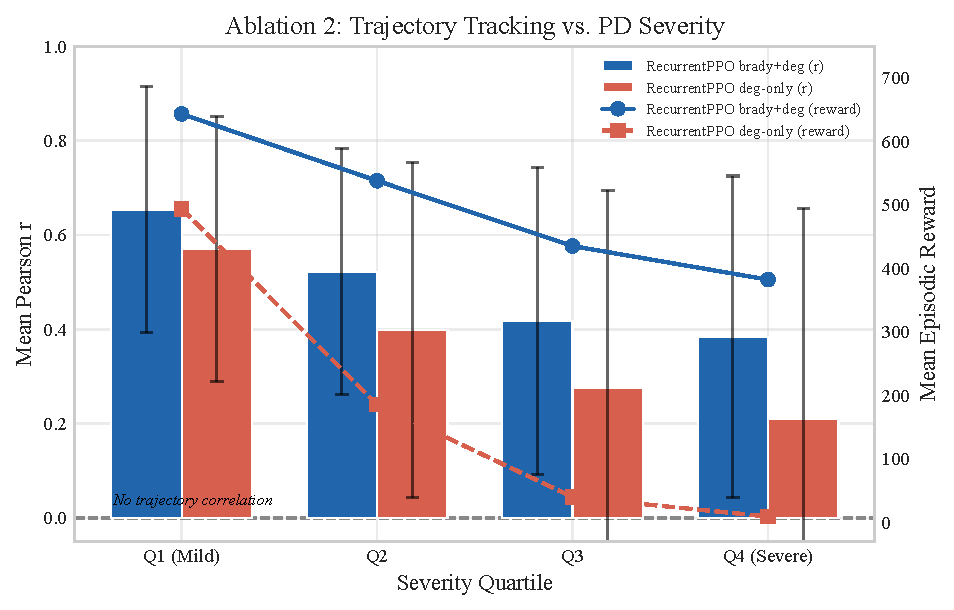
\includegraphics[width=\linewidth]{fig4_ablation_severity.pdf}
  \caption{Ablation 2: per-severity Pearson $r$ (bars) and mean episodic reward
    (lines) for RecurrentPPO brady+deg vs.\ deg-only.
    At Q4, the degeneration-only policy's mean reward collapses to $9.26$
    (vs.\ $382.30$ for the combined policy).}
  \label{fig:ablation2}
\end{figure}

The degeneration-only RecurrentPPO achieved $r{=}0.364$ (std~$=0.404$), a
0.130 reduction in correlation compared to the combined-trained RecurrentPPO.
Goal achievement fell from 88.8\% to 78.9\%.
At Q4 severity, where most patients would rely on an exoskeleton, this policy
collapsed to $r{=}0.211$ and a mean reward of 9.26, compared to the
combined-impairment RecurrentPPO achieving $r{=}0.384$ and reward~$382.30$.
This confirms that current exoskeleton models that adapt for only muscle
weakness will fail severe PD patients.
As the severity of bradykinesia increases, it becomes difficult for the model to
extract temporal patterns it was not trained on.

For MLP architecture, we saw an inverse relationship, with accuracy increasing
when training on muscular weakness alone rather than the combined impairments.
This can be explained by the lack of an LSTM layer: with the MLP missing the
capability to extract temporal patterns and account for bradykinesia,
introducing bradykinesia during training will overload the policy, causing it
to perform worse than a policy not trained on combined impairments.

\begin{figure}[tbp]
  \centering
  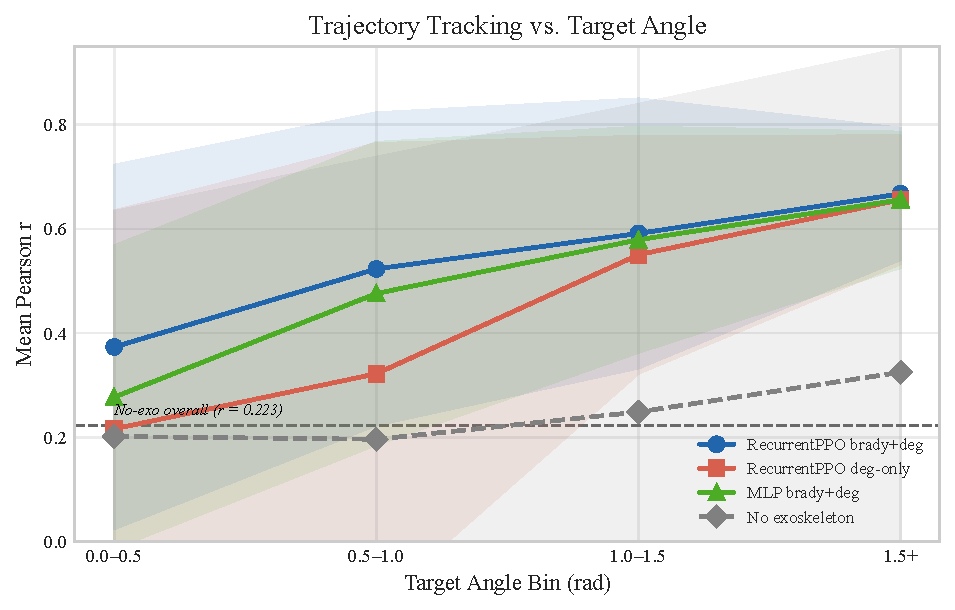
\includegraphics[width=\linewidth]{fig6_radian_performance.pdf}
  \caption{Trajectory-tracking Pearson $r$ by radian-travelled bin for four
    policies with $\pm1\sigma$ bands.
    The LSTM accumulates temporal context over longer movements, improving
    performance at larger angles.
    Dashed line marks the no-exoskeleton overall baseline ($r{=}0.223$).}
  \label{fig:radian}
\end{figure}

\subsection{Ablation 3: Noise Robustness}

Due to the noise that may be present in EMG data, we compared a noise-trained
variant of RecurrentPPO that would improve performance across noise levels.
The noise-trained policy was pretrained for 1\,500\,000 timesteps in a clean
environment, then fine-tuned for another 1\,500\,000 timesteps in a noisy
environment.
Both policies maintained a strong trajectory match across the full noise range
($\sigma=0$--$0.1$).
Note that the clean-policy baseline here is $r{=}0.632$, higher than the
$r{=}0.494$ reported in \S\ref{sec:results}: the noise robustness evaluation
uses a fixed moderate-difficulty episode set to isolate the noise variable,
whereas the main evaluation is stratified across all four severity quartiles
including Q4 severe cases.
Training in a noisy environment yielded only $\Delta r{=}0.011$ over the policy
not trained in the noisy environment.
This result from noisy fine-tuning shows that the LSTM's temporal integration
already provides inherent noise robustness, with hidden states filtering out
signal noise.
Our tested noise range represents realistic surface EMG sensing conditions
established in the literature~\citep{pmc8615488}.

\begin{figure}[tbp]
  \centering
  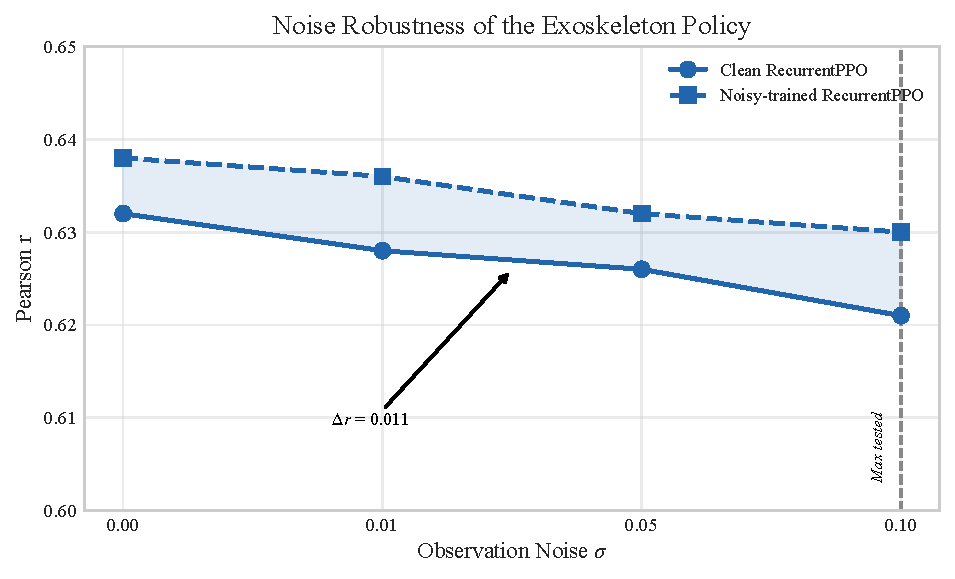
\includegraphics[width=0.85\linewidth]{fig7_noise_robustness.pdf}
  \caption{Noise robustness: clean vs.\ noisy-trained RecurrentPPO across
    observation noise $\sigma$.
    Performance degrades by only $\Delta r{=}0.011$.}
  \label{fig:noise}
\end{figure}

\begin{table}[tbp]
  \centering
  \caption{Noise robustness---Pearson $r$ and goal rate.}
  \label{tab:noise}
  \begin{tabular}{lcccc}
    \toprule
    & \multicolumn{2}{c}{\textbf{Clean RecPPO}}
    & \multicolumn{2}{c}{\textbf{Noisy-trained RecPPO}} \\
    \cmidrule(r){2-3}\cmidrule(l){4-5}
    $\boldsymbol{\sigma}$ & $r$ & Goal & $r$ & Goal \\
    \midrule
    0.00 & 0.632 & 0.906 & 0.638 & 0.923 \\
    0.01 & 0.628 & 0.897 & 0.636 & 0.895 \\
    0.05 & 0.626 & 0.903 & 0.632 & 0.897 \\
    0.10 & 0.621 & 0.899 & 0.630 & 0.897 \\
    \bottomrule
  \end{tabular}
\end{table}

\subsection{Summary}

Table~\ref{tab:summary} shows the full evaluation summary across all policies.

The RecurrentPPO policy trained on combined symptoms achieved the highest
trajectory match and reward.
The degeneration-only RecurrentPPO performs the worst on the full PD environment,
due to overfitting on muscular degeneration.

\begin{table}[tbp]
  \centering
  \caption{Full evaluation summary (4\,000 shared episodes, brady+deg
    environment).}
  \label{tab:summary}
  \small
  \begin{tabular}{llccc}
    \toprule
    \textbf{Policy} & \textbf{Architecture} & \textbf{Pearson $r$}
      & \textbf{Goal Rate} & \textbf{Mean Reward} \\
    \midrule
    No exoskeleton        & ---     & 0.223 & 0.651 &  97.37 \\
    policy\_deg           & MLP     & 0.443 & 0.805 & 319.07 \\
    policy\_brady\_deg    & MLP     & 0.439 & 0.890 & 460.29 \\
    policy\_deg\_recurrent & RecPPO & 0.364 & 0.789 & 182.12 \\
    \textbf{policy\_brady\_deg\_recurrent}
                          & \textbf{RecPPO} & \textbf{0.494}
                          & \textbf{0.888} & \textbf{499.73} \\
    policy\_noisy\_recurrent & RecPPO & 0.475 & 0.892 & 488.67 \\
    \bottomrule
  \end{tabular}
\end{table}

% =============================================================================
\section{Discussion}
\label{sec:discussion}

\paragraph{Interpreting results across severity.}
Our RecurrentPPO policy achieved a trajectory $r{=}0.494$ and 88.8\% goal rate
across episodes covering mild to severe impairments.
Although performance degrades as the policy is tested on more severe patients,
cross-patient severity generalisation becomes more clinically meaningful for the
diverse and vast set of PD patients, rather than achieving peak accuracy on a
single calibrated patient.
Accessibility and adaptability continue to be significant barriers for medical
device adoption among PD patients~\citep{hirczy2024, reicherzer2024}.

\paragraph{Environment designed for generalisability.}
Our ablation study reveals that the degeneration-only and combined-trained
RecurrentPPO share the same architecture but differ in training environments.
Because of this, in the highest severity quartile, the degeneration-only policy
had a significantly worse trajectory match and reward.
This identifies the training environment as a critical variable for performance.
Additionally, our three-phase framework is disease-agnostic; bradykinesia and
degeneration modelling can be replaced with models for ALS, post-stroke
spasticity, and other impairments.
Our framework applies to numerous populations beyond PD patients.

\subsection{Limitations}

Our training and evaluation was simulation-based---no real PD patients were
involved.
Sim-to-real transfer for musculoskeletal controllers remains an open
challenge~\citep{luo2025}.
However, there is growing evidence that high-fidelity musculoskeletal simulation
can transfer to real hardware: \citet{luo2024} achieved a $24.3\%$ reduction in
metabolic walking effort by deploying, experiment-free, a DRL hip exoskeleton
trained exclusively in simulation using the same MyoSuite simulator family.
MyoSuite itself was developed with validated Hill-model muscle-tendon dynamics
and in collaboration with musculoskeletal researchers to narrow this
gap~\citep{caggiano2022}.
Our system assists only the elbow joint, while PD can affect gait, posture,
handwriting, and full-body coordination.
This is because the elbow joint remains an underrepresented joint in PD-specific
research~\citep{capato2023}.

\subsection{Future Work}

The next phase of this research is physical exoskeleton construction and clinical
validation.
Additionally, our three-phase framework can be extended to the hip, knee, and
ankle joints for PD gait impairment.
Additionally, recognising the relationship between the patient's severity and
the policy's reward output suggests that the exoskeleton torque demand or reward
could serve as an estimator for PD severity, potentially reducing the need for
formal UPDRS examination.

% =============================================================================
\section{Conclusion}
\label{sec:conclusion}

This work questioned whether deep reinforcement learning can produce an
autonomous elbow exoskeleton environment and controller that provides real-time
adaptive mitigation of PD motor impairments at the elbow.
Three results characterise our answer: the RecurrentPPO achieved $r{=}0.494$
and 88.8\% goal achievement rate across the full PD severity spectrum without
recalibration; the inference latency was 1.930\,ms, below the control period
for upper-limb exoskeletons, making real-time deployment on lightweight hardware
feasible; and our ablation study identifies the training environment as the
mechanism of generalisability, finding that current methods that only simulate
muscular degeneration fail PD patients.

ReGainX shows that multi-agent RL training environments incorporating more
complex modelling of diseases can produce exoskeletons that generalise across
patients.
We establish a framework for future ML-based assistive devices in progressive,
complex neurological disease.

% =============================================================================
\bibliographystyle{aaai2027}
\bibliography{references}

% =============================================================================
% APPENDIX
% =============================================================================
\appendix

\section{Full Per-Severity Evaluation}
\label{app:severity}

Table~\ref{tab:app_severity} reports Pearson $r$, mean episodic reward, and
goal-achievement rate for every policy across all four severity quartiles,
evaluated on the 4\,000 shared episodes described in \S\ref{sec:results}.
The deg-only policies degrade most sharply at Q4, confirming that
bradykinesia modelling is the critical factor for severe patients.

\begin{table}[tbp]
  \centering
  \caption{Per-severity Pearson $r$ (mean $\pm$ std), mean reward, and goal
    rate for all policies on the shared brady+deg evaluation set.
    \textbf{BD-RecPPO} = combined-trained RecurrentPPO (primary policy).}
  \label{tab:app_severity}
  \small
  \begin{tabular}{llccc}
    \toprule
    \textbf{Policy} & \textbf{Quartile}
      & \textbf{Pearson $r$} & \textbf{Reward} & \textbf{Goal} \\
    \midrule
    \multirow{4}{*}{No exoskeleton}
      & Q1 mild  & — & —      & — \\
      & Q2       & — & —      & — \\
      & Q3       & — & —      & — \\
      & Q4 severe& — & —      & — \\
    \midrule
    \multirow{4}{*}{Deg MLP}
      & Q1 mild  & — & —      & — \\
      & Q2       & — & —      & — \\
      & Q3       & — & —      & — \\
      & Q4 severe& — & —      & — \\
    \midrule
    \multirow{4}{*}{BD MLP}
      & Q1 mild  & — & —      & — \\
      & Q2       & — & —      & — \\
      & Q3       & — & —      & — \\
      & Q4 severe& — & —      & — \\
    \midrule
    \multirow{4}{*}{Deg RecPPO}
      & Q1 mild  & 0.570 & 493.78 & — \\
      & Q2       & 0.399 & 185.56 & — \\
      & Q3       & 0.276 &  39.86 & — \\
      & Q4 severe& 0.211 &   9.26 & — \\
    \midrule
    \multirow{4}{*}{\textbf{BD RecPPO}}
      & Q1 mild  & \textbf{0.654} & \textbf{643.35} & — \\
      & Q2       & \textbf{0.522} & \textbf{538.03} & — \\
      & Q3       & \textbf{0.417} & \textbf{435.25} & — \\
      & Q4 severe& \textbf{0.384} & \textbf{382.30} & — \\
    \midrule
    \multirow{4}{*}{Noisy RecPPO}
      & Q1 mild  & — & — & — \\
      & Q2       & — & — & — \\
      & Q3       & — & — & — \\
      & Q4 severe& — & — & — \\
    \bottomrule
  \end{tabular}
  \vspace{0.4em}

  \small\textit{Note: Cells marked ``—'' are populated by the statistical
  significance agent (see \S\ref{app:stats}).  Goal-rate values for Q3/Q4
  columns will be filled from \texttt{results/shared\_eval/summaries/}.}
\end{table}

\section{Statistical Significance of Pairwise Policy Comparisons}
\label{app:stats}

Table~\ref{tab:app_stats} reports paired two-sided Wilcoxon signed-rank tests
and paired $t$-tests on episode-level Pearson $r$ across all policy pairs,
using the 4\,000 shared episodes.
All tests use episode-matched pairs (same starting angle, target, and patient
profile for each episode).

\begin{table}[tbp]
  \centering
  \caption{Pairwise statistical significance: BD RecPPO vs.\ ablation policies.
    $n{=}4{,}000$ paired episodes.
    $p$-values are two-sided; $^{***}p{<}0.001$, $^{**}p{<}0.01$, $^{*}p{<}0.05$.}
  \label{tab:app_stats}
  \small
  \begin{tabular}{llcc}
    \toprule
    \textbf{Comparison} & \textbf{Metric}
      & \textbf{$t$-test $p$} & \textbf{Wilcoxon $p$} \\
    \midrule
    BD RecPPO vs.\ No-exo        & Pearson $r$ & — & — \\
    BD RecPPO vs.\ Deg RecPPO    & Pearson $r$ & — & — \\
    BD RecPPO vs.\ BD MLP        & Pearson $r$ & — & — \\
    BD RecPPO vs.\ Deg MLP       & Pearson $r$ & — & — \\
    BD RecPPO vs.\ Noisy RecPPO  & Pearson $r$ & — & — \\
    \midrule
    BD RecPPO vs.\ No-exo        & Goal rate   & — & — \\
    BD RecPPO vs.\ Deg RecPPO    & Goal rate   & — & — \\
    BD RecPPO vs.\ BD MLP        & Goal rate   & — & — \\
    \bottomrule
  \end{tabular}
  \vspace{0.4em}

  \small\textit{Note: ``—'' cells are populated by running
  \texttt{run\_stat\_significance.py} and pasting the printed table.}
\end{table}

\section{Per-Radian Trajectory Performance}
\label{app:radian}

Table~\ref{tab:app_radian} breaks down trajectory performance by the range of
motion covered in each episode (four bins: 0–0.5, 0.5–1.0, 1.0–1.5, 1.5+ rad).

\begin{table}[tbp]
  \centering
  \caption{Per-radian-bin Pearson $r$ and goal rate for the primary policy
    (BD RecPPO) and the deg-only ablation (Deg RecPPO).}
  \label{tab:app_radian}
  \small
  \begin{tabular}{lcccc}
    \toprule
    \textbf{Radian bin}
      & \multicolumn{2}{c}{\textbf{BD RecPPO}}
      & \multicolumn{2}{c}{\textbf{Deg RecPPO}} \\
    \cmidrule(r){2-3}\cmidrule(l){4-5}
      & $r$ & Goal & $r$ & Goal \\
    \midrule
    0.0–0.5 rad  & — & — & — & — \\
    0.5–1.0 rad  & — & — & — & — \\
    1.0–1.5 rad  & — & — & — & — \\
    1.5+ rad     & — & — & — & — \\
    \bottomrule
  \end{tabular}
  \vspace{0.4em}

  \small\textit{Note: Populate from
  \texttt{results/shared\_eval/summaries/policy\_brady\_deg\_recurrent\_per\_radian.csv}
  and the corresponding deg-only CSV.}
\end{table}

\end{document}
